\documentclass[]{article}
\usepackage{graphicx}
\usepackage[spanish]{babel}
\usepackage[a4paper, top=2.5cm, bottom=2.5cm, left=3cm, right=3cm]{geometry}
\usepackage[hidelinks]{hyperref}
\usepackage[T1]{fontenc}
\usepackage{xcolor}
\usepackage{float}
\usepackage{circuitikz}
\usepackage{listings}

\definecolor{miverde}{rgb}{0,0.6,0}

\lstset{basicstyle=\ttfamily,
  showstringspaces=false,
  commentstyle=\color{red},
  keywordstyle=\color{blue}
}

\lstdefinestyle{shell}{
    language=bash,
    backgroundcolor=\color{gray!2},     % Color de fondo
    basicstyle=\ttfamily,               % Tipo y tamaño de fuente
    keywordstyle=\color{blue}\bfseries, % Color para palabras clave
    stringstyle=\color{miverde},        % Color para cadenas
    commentstyle=\color{red},           % Color para comentarios
    showspaces=false,                   % No mostrar espacios
    showstringspaces=false,             % No mostrar espacios en las cadenas
    frame=single,                       % Poner un marco alrededor del código
    breaklines=true,                    % Romper las líneas largas
    captionpos=b,                       % Posición del caption
    tabsize=4,                          % Tamaño de las tabulaciones
    escapeinside={\%*}{*)},             % Para incluir código LaTeX en los listings
    morekeywords={self}                 % Palabras clave adicionales
}
\lstset{basicstyle=\ttfamily}
\lstset{
    inputencoding=utf8,
    extendedchars=true,      % Permitir caracteres extendidos (acentos)
    literate=%
        {á}{{\'a}}1 {Á}{{\'A}}1
        {é}{{\'e}}1 {É}{{\'E}}1
        {í}{{\'i}}1 {Í}{{\'I}}1
        {ó}{{\'o}}1 {Ó}{{\'O}}1
        {ú}{{\'u}}1 {Ú}{{\'U}}1
}
\lstset{style=shell}

\usetikzlibrary{positioning}

%title
\title{Guía para la instalación de Git}

\author{Manuel Gómez-Plana Rodríguez}

\begin{document}

\begin{titlepage}
    \centering
    {
        
\includegraphics[width=0.2\textwidth]{./static/eps_logo.png}\\
        \huge Guía para la instalación de Git y Github\\
        \vspace{0.5cm}
        \Large Comisión de Tecnología y Servicios (CTS)\\
        \Large Delegación EPS\\
        \vspace{12.5cm}
    }

    \textbf{Autores:}\\
    \vspace{0.2cm}
    Manuel Gómez-Plana Rodríguez (NIA: 100472310, e-mail: 100472310@alumnos.uc3m.es)\\
    \vspace{0.5cm}
\end{titlepage}
\newpage

\renewcommand{\contentsname}{\centering Índice}
\tableofcontents
\listoffigures

\newpage
\section{Introducción}
Este documento sirve como guía para la instalación de la herramienta de control de versiones \textbf{Git} y el uso de Github para gestionar repositorios de manera básica. A lo largo del mismo, se encuentran varios apartados donde se explican como instalar dicha herramienta en varios sistemas operativos.\\

Este documento está reservado para los integrantes de la Delegación deDestudiantes de la Escuela Politécnica Superior de la Universidad Carlos III de Madrid. Es por ello que, antes de compartir este documento con terceros se deberá contactar con los autores, presentes en la portada.

\newpage
\section{Instalación de Git}
Este apartado se divide en cuatro subapartados, cubriendo los sistemas operativos principales. 

\subsection{Instalación en Linux - Compatibilidad con Debian}
Lo normal es que Git suela estar instalado en Linux, pero, si no lo está, la instalación de Git en las distribuciones de Linux compatibles con Debian sigue los siguientes pasos:

\begin{enumerate}
    \item Abre la terminal de Linux y ejecuta los siguientes comandos:
    \begin{lstlisting}
sudo apt-get update         # actualiza los paquetes 
sudo apt-get install git    # instala git
    \end{lstlisting}
    \item Verifica la instalación de git mediante el comando:
    \begin{lstlisting}
git --version # comprueba que git esta instalado
    \end{lstlisting}
\end{enumerate}

\subsection{Instalación en Linux - Fedora (yum/dnf)}
Lo normal es que Git suela estar instalado en Linux, pero, si no lo está, la instalación de Git en las distribuciones de Linux no compatibles con Debian, como Fedora, sigue los siguientes pasos:

\begin{enumerate}
    \item Abre la terminal de Linux y ejecuta los siguientes comandos:
    \begin{enumerate}
        \item Si usas dnf:
        \begin{lstlisting}
sudo dnf install git    # instala git
        \end{lstlisting}

        \item Si usas yum:
        \begin{lstlisting}
sudo yum install git    # instala git
        \end{lstlisting}
    \end{enumerate}
    \item Verifica la instalación de git mediante el comando:
    \begin{lstlisting}
git --version # comprueba que git esta instalado
    \end{lstlisting}
\end{enumerate}

\subsection{Instalación en Windows}
Para Windows, es tan simple como \textcolor{blue}{\href{https://gitforwindows.org/}{descargar el instalador de Git}} y, una vez descargado, ejecutarlo y pulsar el botón \textit{Next} hasta que aparezca el botón \textit{Finish}.

\subsection{Instalación en MacOS}
Existe una posibilidad de que Git esté preinstalado en MacOS, pero, si no lo está, simplemente hay que \textcolor{blue}{\href{https://sourceforge.net/projects/git-osx-installer/files/}{descargar el instalador oficial para MacOS}} y seguir los pasos del instalador hasta que acabe la instalación. 

\newpage
\section{Creación de la cuenta en Github}
Github es la web desde donde podemos crear los repositorios que clonaremos en nuestra máquina local a través de Git. Es necesario tener una cuenta en Github para poder empezar a usar Git, por ello, hay que hacerse una cuenta en la web. Para ello, sigue los siguientes pasos:

\begin{enumerate}
    \item Dirígete a \textcolor{blue}{\href{https://github.com/}{la web de Github}}
    \item Haz click en el botón para crear una cuenta, \textit{Sign Up}, situado en la esquina superior derecha:
    \item Introduce el e-mail que vas a usar en la cuenta. Se \textbf{recomienda fuertemente} usar el correo de la universidad, ya que con él podrás acceder a GitHub Pro.
    \item Crea una nueva contraseña.
    \item Introduce tu nombre de usuario.
    \item Introduce el código enviado a tu correo.
\end{enumerate}

Una vez hayas creado la cuenta, en la terminal de tu ordenador, emplea los siguientes comandos para guardar la información de tu cuenta:

\begin{lstlisting}
# Usa el nombre de usuario de tu cuenta
git config --global user.name "Tu nombre"
# Usa el correo de tu cuenta
git config --global user.email "ejemplo@email.com"
\end{lstlisting}

\newpage
\section{Usar Git}
Una vez creada la cuenta de Github e instalado Git, hay que seguir una serie de pasos para poder empezar a usar Git. Este apartado se divide según como se quiera usar Git.

\subsection{Git por línea de comandos}
Si quieres usar git en la terminal de tu sistema operativo, sigue los siguientes pasos:

\begin{enumerate}
    \item \textbf{Generar la clave ssh}
    
    Primero, has de generar una clave ssh con la que poder conectar tu cuenta de Github con Git. Para ello, abre una terminal (en \textbf{Windows} abre Git Bash) y copia el siguiente comando:

    \begin{lstlisting}
# Usa el correo de tu cuenta de Github
ssh-keygen -t ed25519 -C "your_email@example.com"
    \end{lstlisting}

    Rellena los campos que te pida, como la carpeta donde guardar las claves o la \textit{passphrase} (contraseña) que usar cuando hagas algún comando (la contraseña es opcional, pulsa enter para dejarla vacía).
    
    \item \textbf{Copiar la clave ssh en Github}
    
    Accede a la web de \textcolor{blue}{\href{https://github.com/}{Github}} y ve a las opciones haciendo click en el menú superior derecha:

    \begin{figure}[H]
        \centering
        
\includegraphics[width=0.3\textwidth]{./static/github_1.png}
        \caption{Acceder a la configuración de Github}
    \end{figure}

    Luego, accede a la sección de las claves shh.
    \begin{figure}[H]
        \centering
        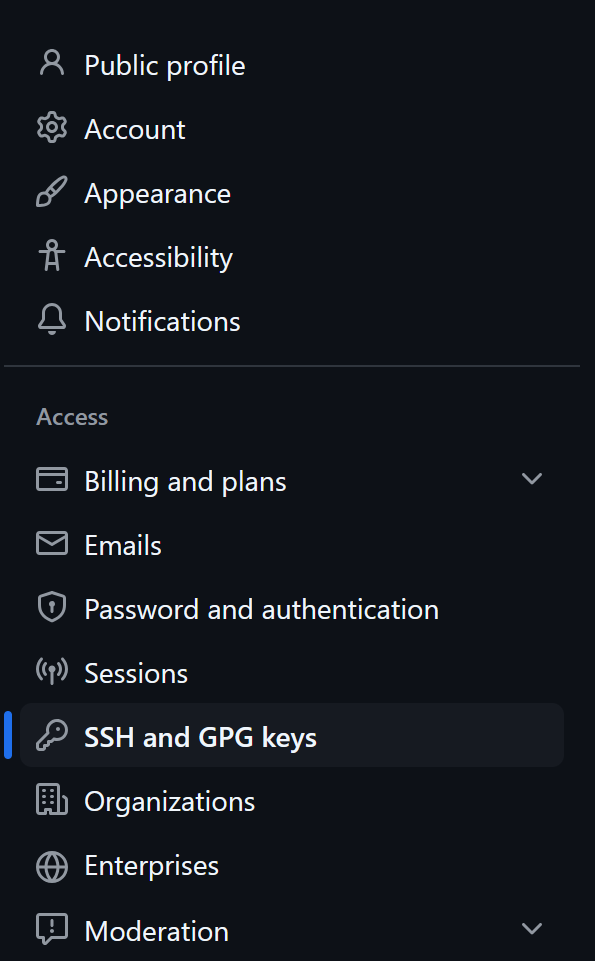
\includegraphics[width=0.3\textwidth]{./static/github_2.png}
        \caption{Acceder a las claves ssh de Github}
    \end{figure}

    Una vez que te encuentres en esta página, haz click en el botón azul para añadir una nueva clave ssh y copia el contenido de la clave pública (.pub) que acabas de crear.
\end{enumerate}

\subsection{Git con Interfaz en los IDE}
Si usas algún IDE para programar, Visual StudioCode o PyCharm, por ejemplo, es recomendable que busques la documentación de los mismos, ya que los métodos para usar Github en una interfaz gráfica para cada uno de ellos es propio. Es por ello que aquí hay recopiladas algunas guías para usar Github con una interfaz en los IDE's más comunes:

\begin{itemize}
    \item \textcolor{blue}{\href{https://www.jetbrains.com/help/pycharm/github.html}{PyCharm}}
    \item \textcolor{blue}{\href{https://code.visualstudio.com/docs/sourcecontrol/github}{VSCode}}
\end{itemize}
\end{document}